% 2022 University of Pennsylvania PhD Dissertation LaTeX Template v.20221216
% This template aims to fulfill University formatting requirements when one follows the instructions, resolves errors and warnings, and does not edit the style file or font size. Consult https://provost.upenn.edu/formatting-faqs for the most up-to-date requirements and policies.
%-------------------------------------------
% We welcome your feedback on the template https://upenn.libwizard.com/f/dissertationlatextemplatefeedback
%-------------------------------------------
% The template requires TeX Live 2022 and is optimized for pdfLaTeX and the LaTeX editor Overleaf. Other LaTeX editing programs may require you to compile the document more than once. It is adapted from the Penn Biostat LaTeX Template modified from Dissertation Template for Wharton PhD Candidates in LaTeX. Portions of the text are reprinted or adapted with permission from Ratcliffe SJ. (2017) Penn Biostat LaTeX Template: PhD dissertation. https://dbe.med.upenn.edu/biostat-research/Dissertation_template

%%%%%%%%%%%%%%%%%%%%%%%%%%%%%%%%%%%%%%%%%%%%%%%%
%%%%%%%%%%%%%%%%%%%%%%%%%%%%%%%%%%%%%%%%%%%%%%%%
\documentclass[11pt]{report}
\usepackage{upennstyle} % You may add additional packages below this line. Overleaf will warn you if your packages conflict with the template packages. See Chapter 1 for more information.

%-------------------------------------------
% Citation and bibliography commands. Edit as needed.
\usepackage[nonamebreak,round]{natbib}
\bibliographystyle{plainnat}
%-------------------------------------------

%%%%%%%%%%%%%%%%%%%%%%%%%%%%%%%%%%%%%%%%%%%%%%%%
%%%%%%%%%%%%%%%%%%%%%%%%%%%%%%%%%%%%%%%%%%%%%%%%
% PLEASE FOLLOW THE INSTRUCTIONS IN THE CODE COMMENTS
% To uncomment a line of code, remove the % at the beginning of the line
% To comment out a line of code, add a % at the beginning of the line
%%%%%%%%%%%%%%%%%%%%%%%%%%%%%%%%%%%%%%%%%%%%%%%%
%%%%%%%%%%%%%%%%%%%%%%%%%%%%%%%%%%%%%%%%%%%%%%%%

%%%%% PRELIMINARY PAGES %%%%%
%-------------------------------------------
%%%% TITLE PAGE
% Edit the text between curly braces {} relevant to your dissertation.
\title{TITLE IN ALL CAPS}
\author{Author's Name as in Path@Penn}
%\specialization{Field of Specialization} % If you are in Romance Languages or Managerial Science and Applied Economics (Wharton), uncomment this line and edit the text between the {}. If you do, you will also need to edit lines 71 and 72.
\gradgroup{Official Graduate Group Name} % See https://provost.upenn.edu/phd-graduate-groups for names
\date{YEAR} % Enter current four-digit year
\supervisor{Supervisor's Typed Name}
\supervisortitle{Full Faculty Title and Affiliation}
%\cosupervisor{Co-supervisor's Typed Name} % If applicable, uncomment this line and edit the text between the {}. If you do, you will also need to edit line 39. 
%\cosupervisortitle{Full Faculty Title and Affiliation} % If applicable, uncomment this line and edit the text between the {}. If you do, you will also need to edit line 38.
\gradchair{Graduate Group Chairperson's Typed Name, Full Faculty Title}
\committee{Committee Member's Typed Name, Full Faculty Title and Affiliation}
\committee{Committee Member's Typed Name, Full Faculty Title and Affiliation}
\committee{Committee Member's Typed Name, Full Faculty Title and Affiliation} % If applicable, comment out or duplicate this line to remove or add a committee member
%-------------------------------------------

%%%% OPTIONAL COPYRIGHT NOTICE
\authorlegal{Author’s Full Legal Name} % To opt out of copyrighting your dissertation, uncomment this line. If you do, you will also need to edit line 76.
%-------------------------------------------
%\cclicense{Name of Selected Creative Commons License} % If applicable, uncomment this line and edit the text between the {}. If you do, you will also need to edit lines 51, 76, and 78.
%-------------------------------------------
%\cclicenseurl{URL of selected Creative Commons License} % If applicable, uncomment this line and edit the text between the {}. If you do, you will also need to edit lines 49, 76, and 78.
%-------------------------------------------

%%%% OPTIONAL DEDICATION
\dedication{Write your dedication text in italics here.} % If not applicable, comment out this line to hide the optional dedication page. If you do, you will also need to edit line 82.
%-------------------------------------------

%%%% OPTIONAL ACKNOWLEDGEMENT
\acknowledgement{Write your acknowledgement text here.} % If not applicable, comment out this line to hide the optional acknowledgement page. If you do, you will also need to edit line 86.
%-------------------------------------------

%%%% ABSTRACT
\abstract{Write your abstract text here.} % Write your abstract between the {}
%-------------------------------------------

%%%% OPTIONAL PREFACE
%\preface{Write your preface text here.} % If applicable, uncomment this line and write your preface between the {}. If you do, you will also need to edit line 101.
%-------------------------------------------

\begin{document}
\maketitle % If you are in Romance Languages or Managerial Science and Applied Economics (Wharton), comment out this line. If you do, you will also need to edit lines 33 and 72.
%\makespecializationtitle % If you are in Romance Languages or Managerial Science and Applied Economics (Wharton), uncomment this line. If you do, you will also need to edit lines 33 and 71.
\setcounter{page}{2}

%%%% OPTIONAL COPYRIGHT NOTICE
\makecopyright % If not applicable, comment out this line to hide the optional traditional copyright notice page. If you do, you will also need to edit line 47.
%-------------------------------------------
%\makecreativecommons % If applicable, uncomment this line to insert the optional Creative Commons License copyright notice page. If you do, you will also need to edit lines 49, 51, and 76.
%-------------------------------------------

%%%% OPTIONAL DEDICATION PAGE
\makededication % If not applicable, comment out this line to hide the optional dedication page. If you do, you will also need to edit line 55.
%-------------------------------------------

%%%% OPTIONAL ACKNOWLEDGEMENT PAGE
\makeacknowledgement % If not applicable, comment out this line to hide the optional acknowledgment page. If you do, you will also need to edit line 59.
%-------------------------------------------

\makeabstract
\tableofcontents

%%%% OPTIONAL LIST OF TABLES
\clearpage \phantomsection \addcontentsline{toc}{chapter}{LIST OF TABLES} \begin{singlespacing} \listoftables \end{singlespacing}% If not applicable, comment out this line to hide the optional List of Tables
%-------------------------------------------

%%%% OPTIONAL LIST OF ILLUSTRATIONS
\clearpage \phantomsection \addcontentsline{toc}{chapter}{LIST OF ILLUSTRATIONS} \begin{singlespacing} \listoffigures \end{singlespacing}% If not applicable, comment out this line to hide the optional List of Illustrations
%-------------------------------------------

%%%% OPTIONAL PREFACE
%\makepreface % If applicable, uncomment this line to insert the optional preface. If you do, you will also need to edit line 67.
%-------------------------------------------

%%%%% MAIN TEXT %%%%%
\begin{mainf} % The main body of your dissertation starts below this line
\chapter{UNIVERSITY OF PENNSYLVANIA PH.D. DISSERTATION LATEX TEMPLATE}
\section{Introduction}
This template aims to fulfill University format requirements when one follows the instructions, resolves errors and warnings, and does not change the style file or font settings. Your graduate group may have additional formatting requirements like specific citation and bibliography styles.\footnote{If you are using another LaTeX template, please make sure it complies with all University formatting requirements.} Check with your advisor and edit the template as needed. Please consult the Office of the Provost dissertation \textit{\underline{\href{https://provost.upenn.edu/formatting-faqs}{Formatting FAQs}}} for the most up-to-date requirements and policies.

\section{Getting Started}
The template requires TeX Live 2022 and is optimized for pdfLaTeX and the LaTeX editor Overleaf. Other LaTeX editing programs may require you to compile the document more than once. To claim your free Overleaf Pro account, go to the \underline{\href{https://www.overleaf.com/edu/upenn}{Penn Libraries Overleaf Portal}} and click on the green ``Log in through your institution'' button.

Click \underline{\href{https://www.overleaf.com/contact}{here}} if you have a question about Overleaf, and they'll make sure it reaches the right person. Click \underline{\href{https://www.overleaf.com/help/18-how-do-i-use-overleaf}{here}} for their help page to learn how to use Overleaf and LaTeX. See Chapter~\ref{sec:helpfeedback} for additional resources.

\subsection{Packages}
The template automatically loads the packages it requires to function. See the PackagesLoadedbyTemplate.tex file for a complete list of all the packages loaded by the template. You may manually load other packages if you wish, and Overleaf will give you a warning message when you compile your document if your package conflicts with one of the template's packages. If you receive a warning, you can consult the specified package documentation on \underline{\href{https://www.ctan.org}{CTAN}} for a possible resolution.
\newpage
\section{Margins}
\textbf{As of January 2023, the margins must be 1 inch on each side.} Remember to resolve all overfull or underfull warnings to help ensure your dissertation meets the margin requirements.\footnote{This is a common source of errors -- please double check the margins before submitting your final dissertation.} Click \underline{\href{https://www.overleaf.com/learn/how-to/Understanding_underfull_and_overfull_box_warnings\#How_the_Error_Happens}{here}} to learn how to identify and resolve the warnings. Common causes of warnings include 
\begin{itemize}
\item \textbf{LaTeX CANNOT automatically break long mathematical expressions or parenthetical references across multiple lines.} Chapter~\ref{ch:equations} demonstrates two methods for manually splitting equations.
\item You can manually control the hyphenation by using the \verb|\hyphenation{}| hints command. For example, write \verb|\hyphenation{rep-re-sent-a-tive}| in the preamble to tell LaTeX where it can break the word ``representative.''
\item The verbatim environment and the \verb|\verb| command remove LaTeX's formatting controls. There may be instances that require you to manually adjust line breaks.
\item The breaklinks option of the hyperref package is activated, however there may be instances of URLs running into the margins that require your manual intervention.
\end{itemize}

\section{Template Tips}
\subsection{Chapters, sections, and subsections}
Create chapters with the \verb|\chapter| command, sections with the \verb|\section| command, and subsections with the \verb|\subsection| command. If you use the \verb|\MakeUppercase| command to autocapitalize chapter titles, carefully check each title and its table of contents entry for compliance with University formatting requirements. You may wish to split chapters into separate .tex files for easier document management. You can use the \verb|\include{}| command to add the chapters to your main .tex file. Click \underline{\href{https://www.overleaf.com/learn/latex/Management_in_a_large_project\#Inputting_and_including_files}{here}} to learn more.

If a chapter or section title contains math expressions or other symbols, the \verb|hyperref| package may give a PDFDocEncoded warning when you compile your document. Use the \verb|\texorpdfstring| command to edit the corresponding PDF bookmark text to resolve the warning. 
For example, the section title ``Lemurs Wrote $E=mc^2$ in Mud on the Riverbank'' should be coded
\begin{verbatim}
 \section{Lemurs Wrote \texorpdfstring{$E=mc^2$}{E=mc2} in Mud on the Riverbank}   
\end{verbatim}

\subsection{Page orientation}
The template's default page orientation is portrait. Use the landscape environment to create landscape pages. Page number location and margins will automatically update like page~\pageref{fig:landlemur1}.

\section{Getting Help and Giving Feedback} \label{sec:helpfeedback}
Questions about LaTeX?
\begin{itemize}
    \item Click \underline{\href{https://guides.library.upenn.edu/LaTeX}{here}} to connect with LaTeX resources, tutorials, and more.
\end{itemize}
Want to give feedback on the template?
\begin{itemize}
    \item Click \underline{\href{https://upenn.libwizard.com/f/dissertationlatextemplatefeedback}{here}} to share it with us.
\end{itemize}

\section{Acknowledgments}
The University of Pennsylvania Ph.D. Dissertation LaTeX Template was initiated by Dr.~Beth S. Wenger, Associate Dean for Graduate Studies, School of Arts and Sciences. It was developed by Lauren Gala, Penn Libraries with assistance from Dr.~Julia Hartmann and Dr.~Man Cheung Tsui, Department of Mathematics, and Bridget Rothera, Graduate Division School of Arts and Sciences. Portions of the code and text were reprinted or adapted with permission from Ratcliffe S.J. (2017) \underline{\href{https://dbe.med.upenn.edu/biostat-research/Dissertation\_template}{Penn Biostat LaTeX Template: PhD dissertation}} modified from Dissertation Template for Wharton PhD Candidates in LaTeX.

\chapter{\MakeUppercase{Tables and Figures}}
\section{Tables}
The captions of tables inside the table environment (see Table~\ref{extab}) will display in the List of Tables. Use the \verb|\label| to label tables. 
\begin{table}[h]
\begin{center}
\begin{tabular}{cc|c|c|c|c|l}
\cline{3-6}
& & \multicolumn{4}{|c|}{Primes} \\ \cline{3-6}
& & 2 & 3 & 5 & 7 \\ \cline{1-6}
\multicolumn{1}{|c|}{\multirow{2}{*}{Powers}} &
\multicolumn{1}{|c|}{504} & 3 & 2 & 0 & 1 &     \\ \cline{2-6}
\multicolumn{1}{|c|}{}                        &
\multicolumn{1}{|c|}{540} & 2 & 3 & 1 & 0 &     \\ \cline{1-6}
\multicolumn{1}{|c|}{\multirow{2}{*}{Powers}} &
\multicolumn{1}{|c|}{gcd} & 2 & 2 & 0 & 0 & min \\ \cline{2-6}
\multicolumn{1}{|c|}{}                        &
\multicolumn{1}{|c|}{lcm} & 3 & 3 & 1 & 1 & max \\ \cline{1-6}
\end{tabular}
\caption{Example Table}\label{extab}
\end{center}
\end{table}

\section{Figures}
The captions of figures inside the figure environment (see Figure~\ref{fig:lemur1}) will display in the List of Illustrations. Use the \verb|\label| to label figures.\footnote{This also includes photographs, maps, schemes, diagrams, etc.}
\newpage
\begin{figure}[H]
\begin{center}
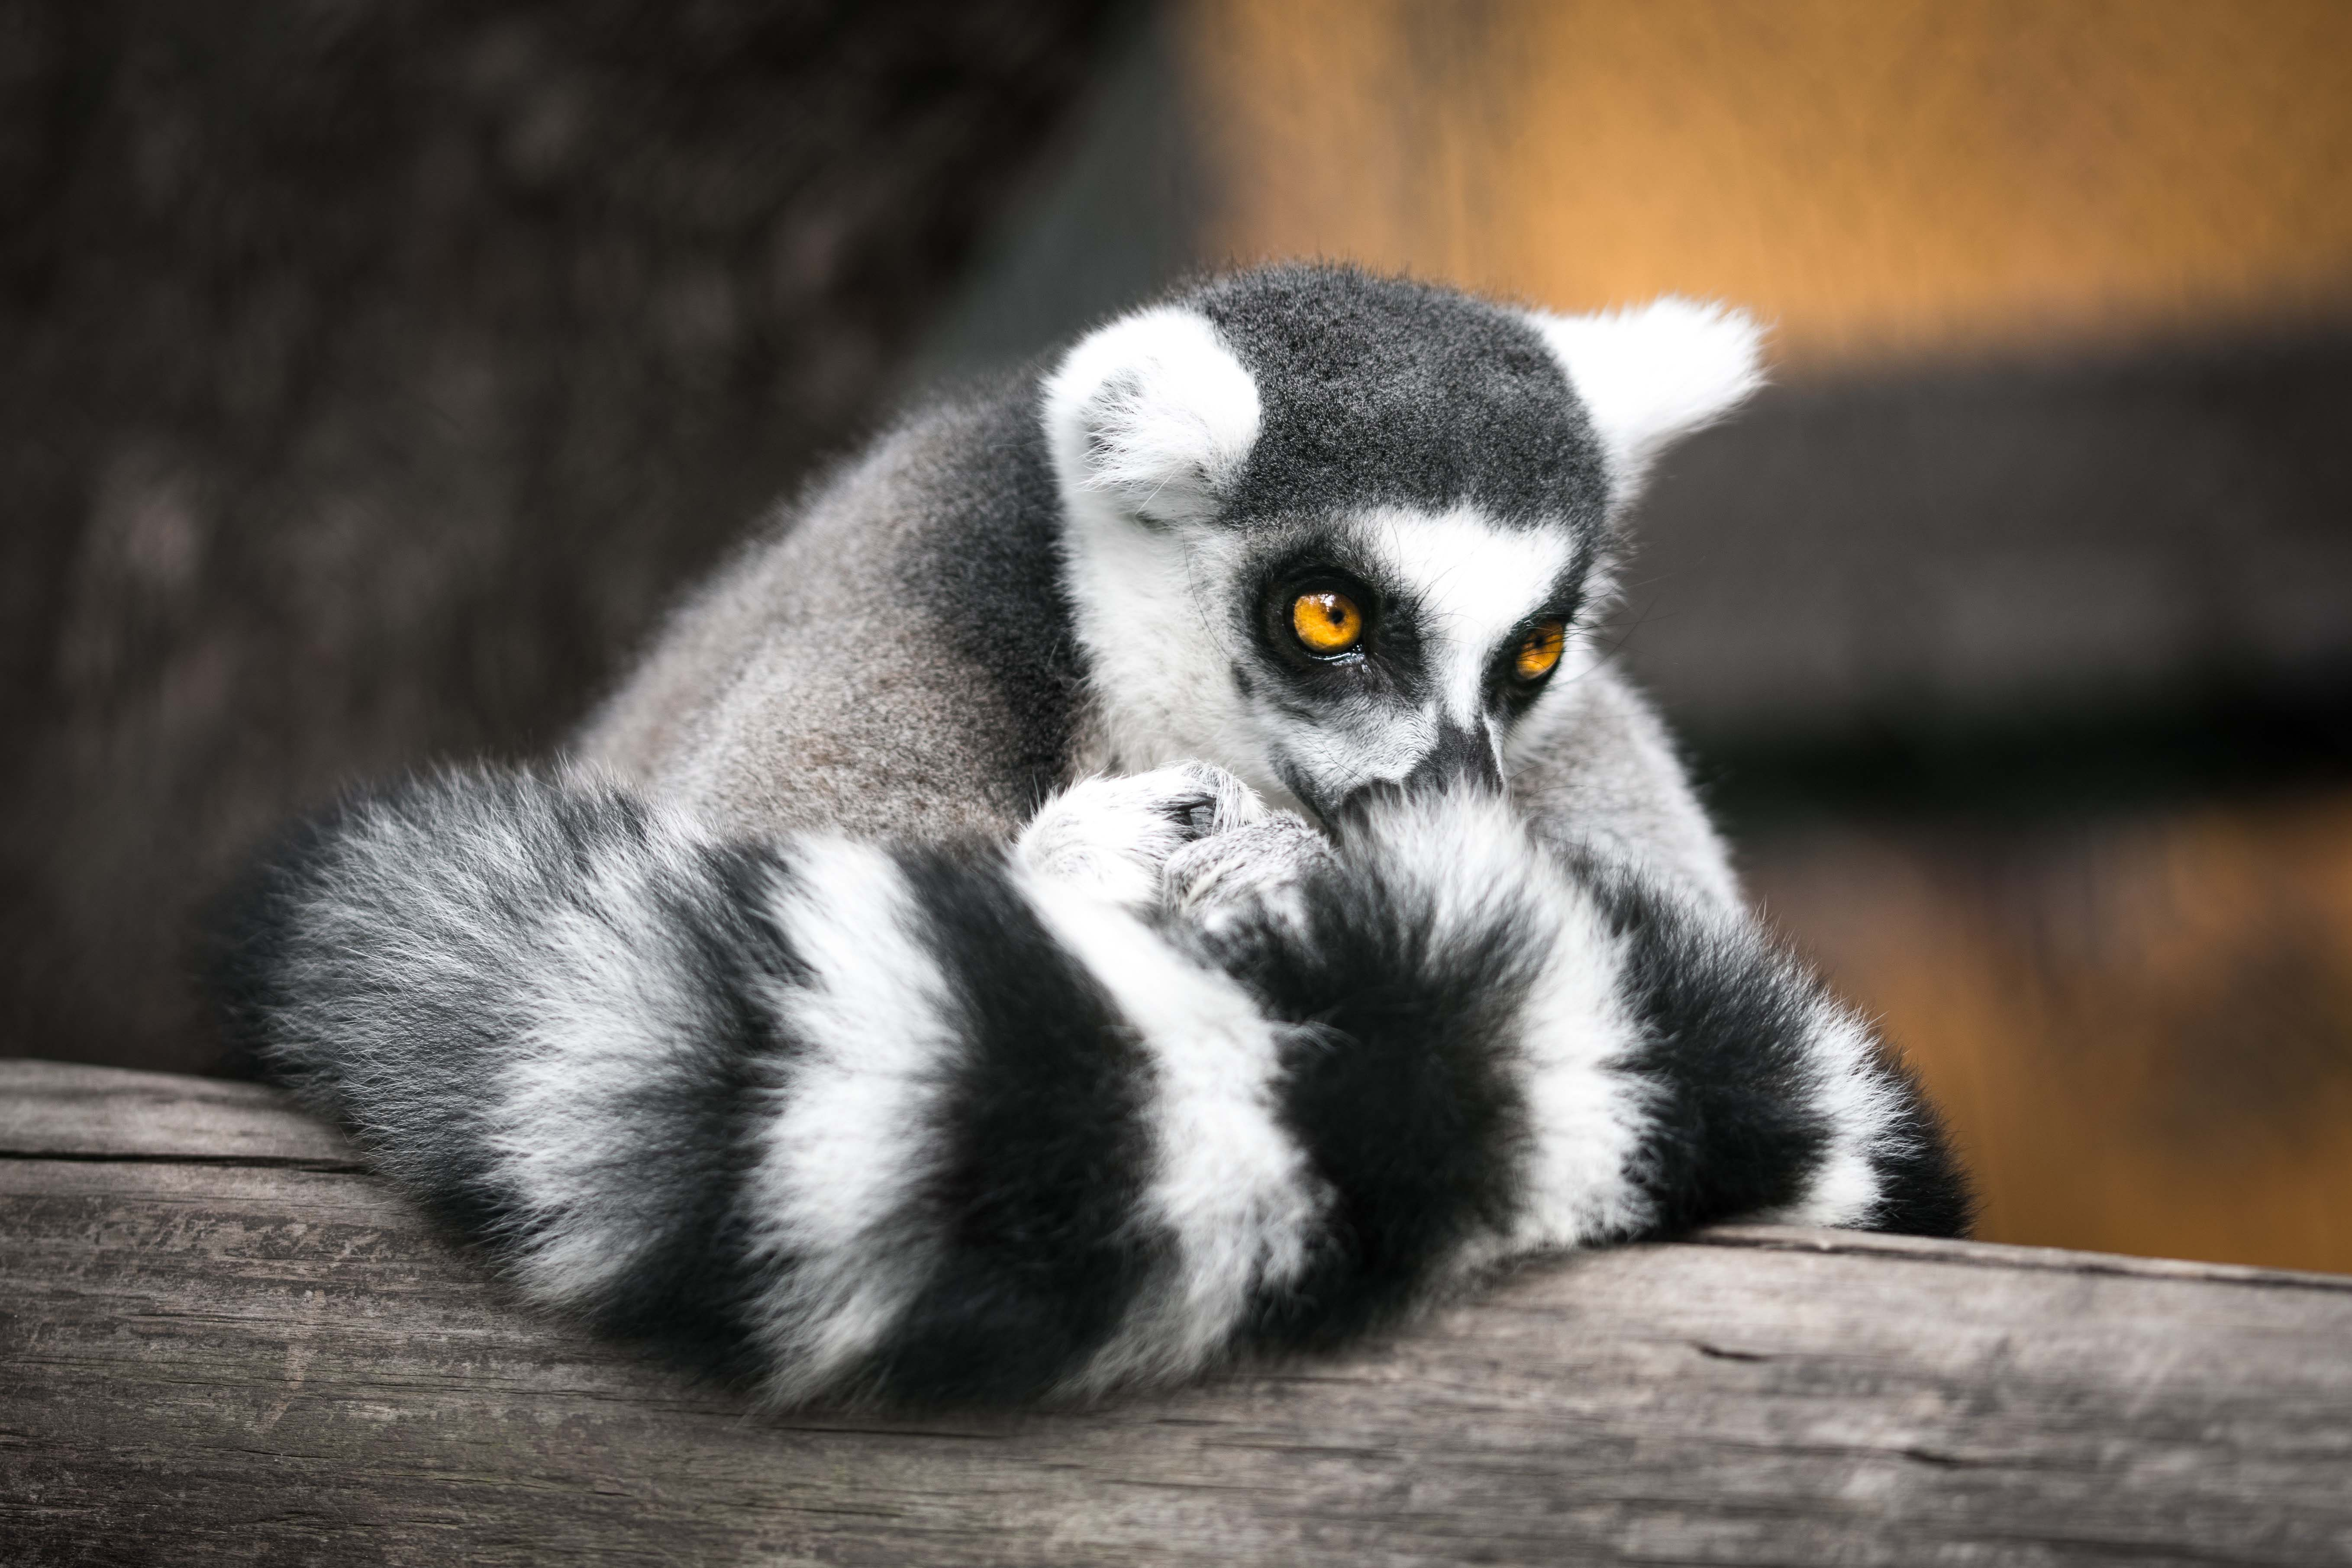
\includegraphics{lemurphoto}
\caption{Lemur photograph} \label{fig:lemur1}
\end{center}
\end{figure}

LaTeX takes into account line and page breaks when determining where to place floating objects like figures and tables on a page. You can override LaTeX's placement decisions by using the float package options. Consult the \underline{\href{https://ctan.org/pkg/float}{float package documentation}} to learn how to gain more control over where and how float objects display.
 
\begin{landscape}
\begin{figure}[H]
\begin{center}
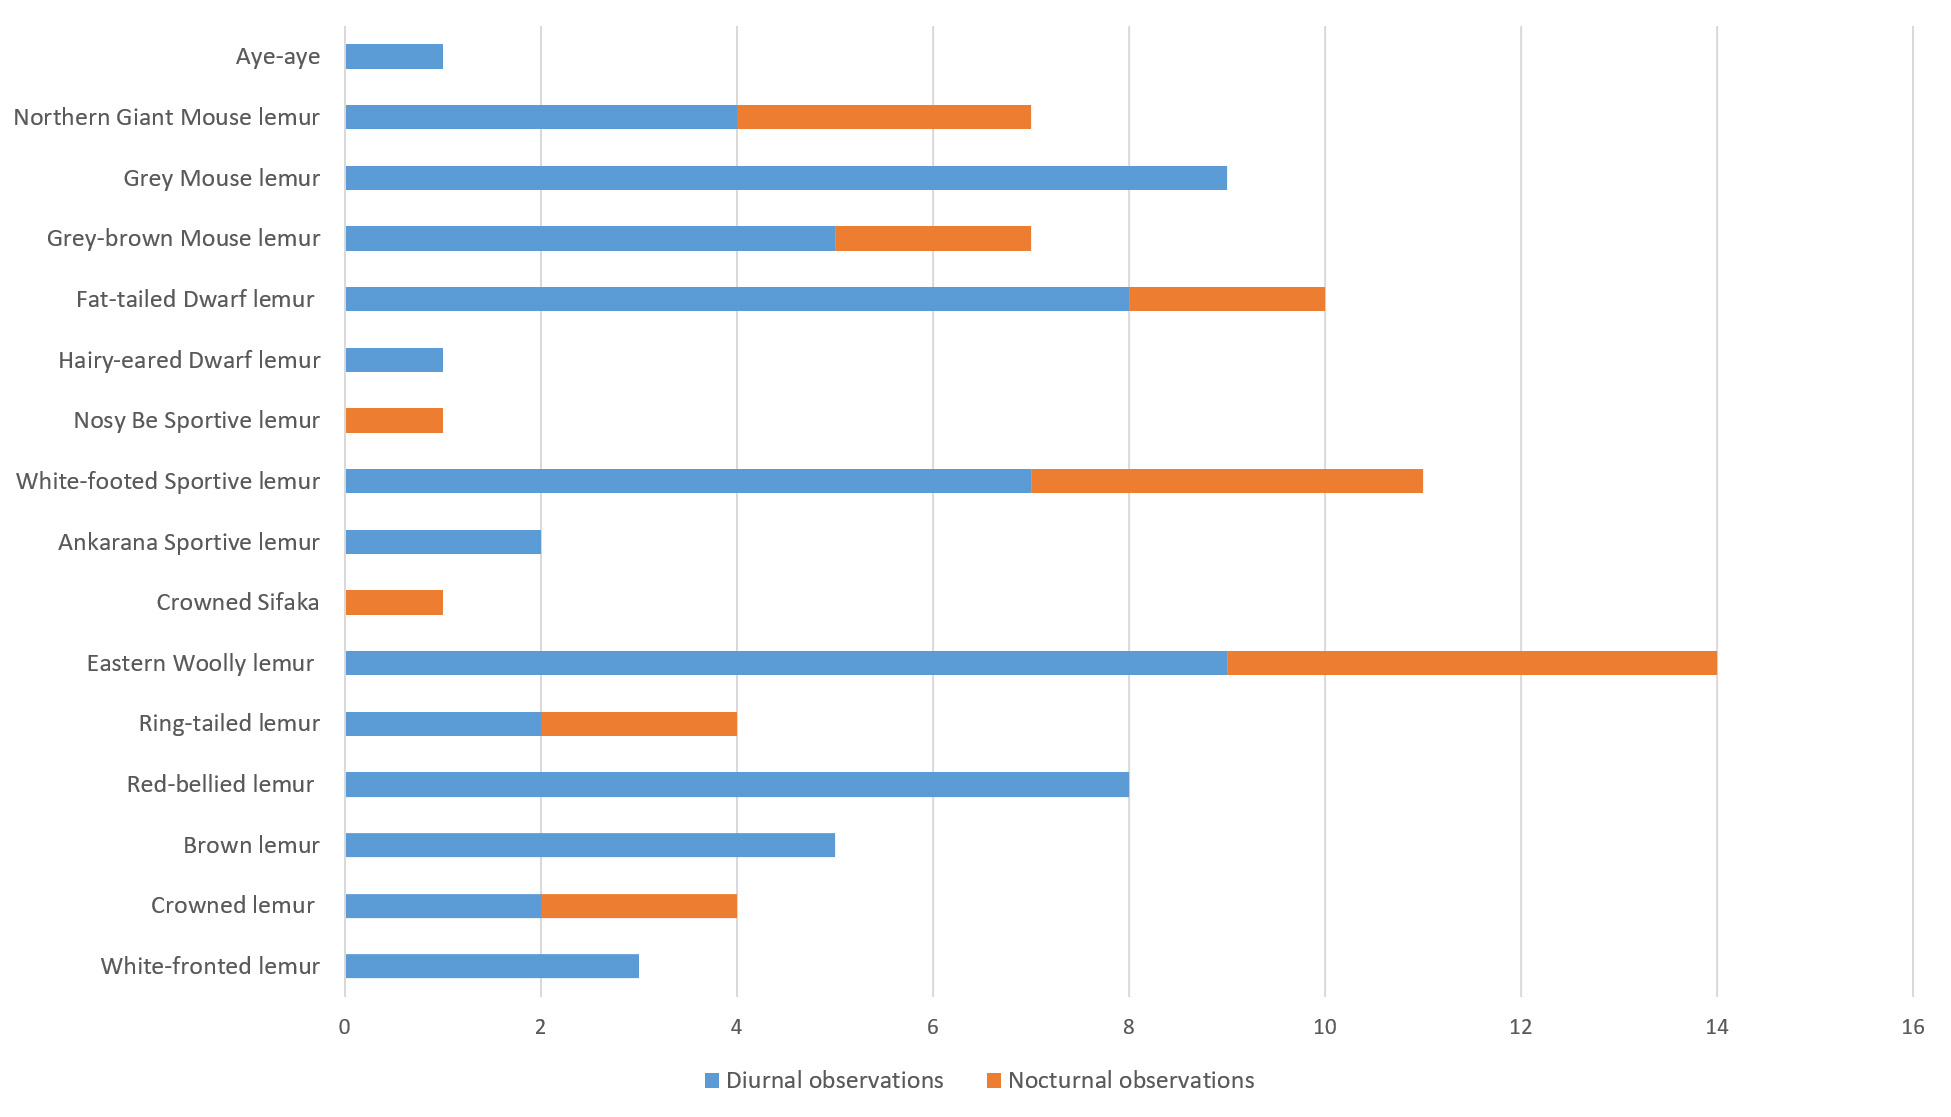
\includegraphics{lemurchart}
\caption{Lemur bar chart on landscape page} \label{fig:landlemur1}
\end{center}
\end{figure}
\end{landscape}

\chapter{\MakeUppercase{Equations}} \label{ch:equations}
The template automatically loads several math packages like amsmath, amssymb, and amsfonts. The split and the multline environments allow you to split an equation over multiple lines. Equation~\ref{eq:split} is written in the split environment, and Equation~\ref{eq:mult} is in the multline environment. Notice the differences in how the two environments align the equations and where they place the equation number.

\begin{equation} \label{eq:split}
\begin{split}
A & = \frac{\pi r^2}{2} \\
 & = \frac{1}{2} \pi r^2
\end{split}
\end{equation}

\begin{multline} \label{eq:mult}
p(x) = 3x^6 + 14x^5y + 590x^4y^2 + 19x^3y^3 + 3x^6 + 14x^5y + 590x^4y^2 + 19x^3y^3\\ 
+ 3x^6 + 14x^5y + 590x^4y^2 + 19x^3y^3- 12x^2y^4 - 12xy^5 + 2y^6 - a^3b^3
\end{multline}

\chapter{\MakeUppercase{Appendices}}
Appendices are optional. Use the \verb|\chapter| command inside the custom \verb|append| environment to insert appendices. Use the \verb|\ref{ }| command to reference appendices in your text.

\chapter{\MakeUppercase{Citations and Bibliography}} \label{ch:citebib}
LaTeX bibliography packages and citation management programs enable you to efficiently cite and format bibliographic references. You can manage bibliographic entries in a separate bibliography database file (*.bib) or you can embed the entries directly into the main .tex file. While the LaTeX template was built for the former approach, you can modify it to accommodate latter.

\section{Getting Started}
Please watch this \underline{\href{https://mediaspace.library.upenn.edu/media/LaTeX+Fundamentals+-+6.1+Citations+\%26+Bibliographies+-+Think+in+LaTeX\%2C+BibTeX\%2C+and+BibLaTeX/1_7dyh4j58}{short video}} to learn the principles underpinning the template bibliography before proceeding.

\section{Default Template Settings}
The commands written in sampledissertation.tex load the natbib package in its preamble and reference the bibliographic entries stored in bibliography.bib.

This is an example inline citation \citep{heard_charles_2020}. 
If you want to cite two publications in one place like \citep{mcgoogan_chasing_2020,wright_for_2014}, write one citation command. You can add a prenote or postnote \citep[p.~78]{lake_white_1979} to a citation.

\section{Customization}
Citation and bibliography formatting commands are written in the main .tex file for your convenience. You can edit the relevant code in the .tex file to produce citation and bibliography styles appropriate for your field. If you wish to make significant to changes to the structure of the bibliography, you may need to edit the bibliof environment defined in upennstyle.sty.

\subsection{Styles and formatting}
The natbib package, selected format and style options, and example citations are for demonstration. In addition to natbib, other packages and accompanying documentation are free to download from \underline{\href{https://www.ctan.org}{CTAN}}. 
Always consult the package documentation for additional citation and bibliography commands and formatting options. Remember that the available commands and styles differ between packages.

\subsection{Embedded bibliography}
You can edit the template to manage your bibliography directly in the .tex file obviating the need for a separate .bib file. Replace the \verb|\bibliography| command in the bibliof environment with the list of bibitems and edit relevant code elsewhere in the template as needed. 

\section{Recommended Resources}
\begin{itemize}
    \item Click \underline{\href{https://guides.library.upenn.edu/LaTeX/cite}{here}} to learn how to manage citations and bibliographies in LaTeX documents
    \item Click \underline{\href{https://www.library.upenn.edu/help-with/tutorials/citation-practices}{here}} to learn citation best practices and how to use citation management programs
    \item Click \underline{\href{https://mediaspace.library.upenn.edu/media/LaTeX+Fundamentals+-+6.2+Citations+\%26+Bibliographies+-+natbib/1_sxrfdv5j}{here}} to watch a short introduction to citing and formatting references with natbib
\end{itemize}

\end{mainf}
%-------------------------------------------

%%%%% OPTIONAL APPENDICES %%%%%
%-------------------------------------------
\begin{append}
\chapter{\MakeUppercase{Title of Appendix A}}
The content of Appendix A begins here. Use the \verb|\chapter| command to insert additional appendices.
\section{Section Name of Appendix A}
Use the \verb|\section| command to create sections.
\chapter{\MakeUppercase{Title of Appendix B}}
The content of Appendix B begins here.
\end{append}
%-------------------------------------------

%%%%% BIBLIOGRAPHY %%%%%
%-------------------------------------------
\begin{bibliof}
%\nocite{*} % If applicable, uncomment this line to display all entries in the .bib file
\bibliography{bibliography}
\end{bibliof}
%-------------------------------------------
\end{document}